% --------------------------------------------------------------
% This is all preamble stuff that you don't have to worry about.
% Head down to where it says "Start here"
% --------------------------------------------------------------
 
\documentclass[12pt]{article}
 
\usepackage[margin=1in]{geometry} 
\usepackage{amsmath,amsthm,amssymb}
\usepackage{mathtools}
\usepackage{upgreek}
\usepackage{algorithm}
\usepackage{comment}
\usepackage[noend]{algpseudocode}
 \usepackage{algpseudocode}
 \usepackage{pgffor}
 \usepackage[document]{ragged2e}
 \DeclarePairedDelimiter\ceil{\lceil}{\rceil}
\DeclarePairedDelimiter\floor{\lfloor}{\rfloor}\newcommand{\N}{\mathbb{N}}
\newcommand{\Z}{\mathbb{Z}}
 
\newenvironment{theorem}[2][Theorem]{\begin{trivlist}
\item[\hskip \labelsep {\bfseries #1}\hskip \labelsep {\bfseries #2.}]}{\end{trivlist}}
\newenvironment{lemma}[2][Lemma]{\begin{trivlist}
\item[\hskip \labelsep {\bfseries #1}\hskip \labelsep {\bfseries #2.}]}{\end{trivlist}}
\newenvironment{exercise}[2][Exercise]{\begin{trivlist}
\item[\hskip \labelsep {\bfseries #1}\hskip \labelsep {\bfseries #2.}]}{\end{trivlist}}
\newenvironment{problem}[2][Problem]{\begin{trivlist}
\item[\hskip \labelsep {\bfseries #1}\hskip \labelsep {\bfseries #2.}]}{\end{trivlist}}
\newenvironment{question}[2][Question]{\begin{trivlist}
\item[\hskip \labelsep {\bfseries #1}\hskip \labelsep {\bfseries #2.}]}{\end{trivlist}}
\newenvironment{corollary}[2][Corollary]{\begin{trivlist}
\item[\hskip \labelsep {\bfseries #1}\hskip \labelsep {\bfseries #2.}]}{\end{trivlist}}
 
\begin{document}
 
% --------------------------------------------------------------
%                         Start here
% --------------------------------------------------------------
 
\title{STAT1234 Assignment x}%replace X with the appropriate number
\author{=-=\\ %replace with your name
} %if necessary, replace with your course titles
 
\maketitle

\begin{question}{EX 10.09} %You can use theorem, exercise, problem, or question here.  Modify x.yz to be whatever number you are proving
Crab Claws
\end{question}
\begin{enumerate}
	\item hahahah
	\item $qt(0.025,df=32) = -2.036933$, the $95\%$ confidence interval is $\mu \pm t_{0.025}(32)*SE = 1.6601 \pm (-2.036933)*0.7889$, which is $(0.05316356,3.267036)$
\end{enumerate}



\begin{question}{EX 10.33}
	IQ Score and Income
\end{question}
\begin{enumerate}
	\item We draw scatter plots for four test scores.
	
	\begin{figure}[!ht]
		\label{Word}
		\caption{Word vs log(Income2005)}
		\centering
		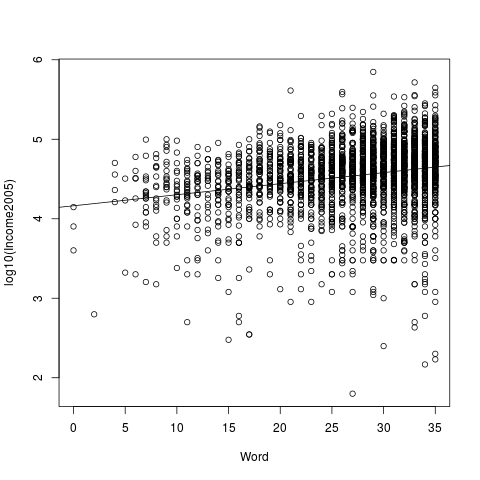
\includegraphics[width=0.5\textwidth]{Word}
	\end{figure}
	
	
	\item from the summary(lm.all), we find that slope for $Arith$ is $0.0121320$, which is bigger than others. And the $p-value$ is $3.34e-07$. We have to reject the null hypothesis that slope is $0$. So we conclude that variable $Arith$ contributes the most. 
	
		
\end{enumerate}
\end{document}
